\documentclass[a4paper, 12pt, one column]{article}

%% Language and font encodings. This says how to do hyphenation on end of lines.
\usepackage[english]{babel}
\usepackage[utf8x]{inputenc}
\usepackage[T1]{fontenc}
% \usepackage[clean]{svg}

%% Sets page size and margins. You can edit this to your liking
\usepackage[top=1.3cm, bottom=2.0cm, outer=2.5cm, inner=2.5cm, heightrounded,
marginparwidth=1.5cm, marginparsep=0.4cm, margin=2.5cm]{geometry}

%% Useful packages
\usepackage{rotating, graphicx} %allows you to use jpg or png images. PDF is still recommended
\graphicspath{ {./images/} }
\usepackage[colorlinks=False]{hyperref} % add links inside PDF files
\usepackage{amsmath}  % Math fonts
\usepackage{amsfonts} %
\usepackage{amssymb}  %
\usepackage{listings}
\usepackage{xcolor}
%\usepackage[margin=0.25in]{geometry}
\usepackage{pgfplots}
\pgfplotsset{width=10cm,compat=1.9}
\usepackage {tikz}
\usetikzlibrary {positioning}

\definecolor{codegreen}{rgb}{0,0.6,0}
\definecolor{codegray}{rgb}{0.5,0.5,0.5}
\definecolor{codepurple}{rgb}{0.58,0,0.82}
\definecolor{backcolour}{rgb}{0.95,0.95,0.92}
\lstdefinestyle{mystyle}{ 
    commentstyle=\color{codegreen},
    keywordstyle=\color{magenta},
    numberstyle=\tiny\color{codegray},
    stringstyle=\color{codepurple},
    basicstyle=\ttfamily\footnotesize,
    breakatwhitespace=false,         
    breaklines=true,                 
    captionpos=b,                    
    keepspaces=true,                 
    numbers=left,                    
    numbersep=0pt,                  
    showspaces=false,                
    showstringspaces=false,
    showtabs=false,                  
    tabsize=1
}

\lstset{style=mystyle}

%% Citation package
\usepackage[authoryear]{natbib}
\bibliographystyle{abbrvnat}
\setcitestyle{authoryear,open={(},close={)}}


\title{Parallel Programmeren: Classificatie met Neurale Netwerken}
\author{Pieter Dilien, Waldo Wautelet}

\begin{document}
\maketitle

\section{Introductie}
In dit verslag zal het paralleliseren van een programma dat een afbeelding kan classificeren besproken worden.
Eerst zal het originele niet-geparalleliseerde programma bekeken worden. Vervolgens zal er ingegaan worden op 
de verbeteringen die er aan het originele programma aangebracht zijn om het parallel te laten functioneren. Ten slotte
zullen de resultaten van de beide programma's vergeleken worden.

\section{Origineel}
Eerst en vooral werd bestudeerd hoe het programma juist werkte. Vervolgens bekeken we welke layers het meeste computing time 
innamen. Dit om te bepalen welke layers nog het meest ruimte voor verbetering hadden. De layertijden van het originele programma
zijn te zien op figuur \ref{layers}.

\noindent
Het is duidelijk dat layers 1, 3, 6, 10, 14, 18, 19, 21 en 22 reeds erg snel zijn. Deze hebben dus minder marge voor verbetering.
Hierdoor keken we naar de overgebleven layers. Het werd snel duidelijk dat deze allemaal gebruikmaken van de convolution\_layer functie.
Het is dan ook deze functie dat gekozen werd om te paralleliseren.

\section{Verbeterd}

\section{Resultaten}

\begin{figure}
  \centering
  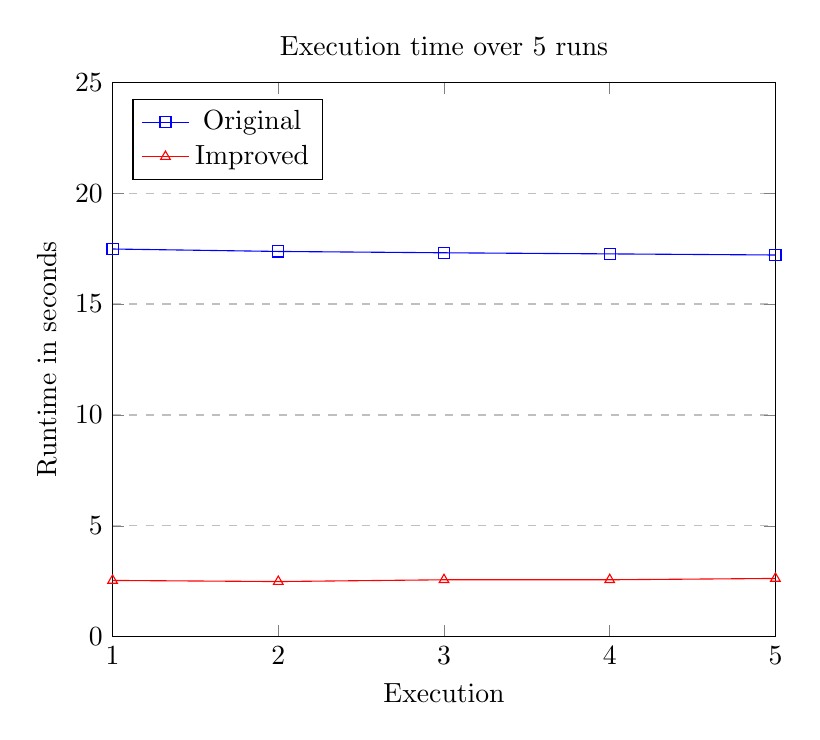
\begin{tikzpicture}
    \begin{axis}[
        title={Execution time over 5 runs},
        xlabel={Execution},
        ylabel={Runtime in seconds},
        xmin=1, xmax=5,
        ymin=0, ymax=25,
        ytick={0,5,10,15,20, 25},
        xtick={1,2,3,4,5},
        legend pos=north west,
        ymajorgrids=true,
        grid style=dashed,
    ]
    
    \addplot[
        color=blue,
        mark=square,
        ]
        coordinates {
          (1, 17.48)(2, 17.37)(3, 17.31)(4, 17.26)(5, 17.21)
        };
    
    \addplot[
        color=red,
        mark=triangle,
        ]
        coordinates {
          (1, 2.54)(2, 2.49)(3, 2.57)(4, 2.57)(5, 2.63)
        };
        \legend{Original, Improved}
    \end{axis}
  \end{tikzpicture}
  \caption{Execution time of original and improved program}
  \label{general}
\end{figure}

\begin{figure}
  \centering
  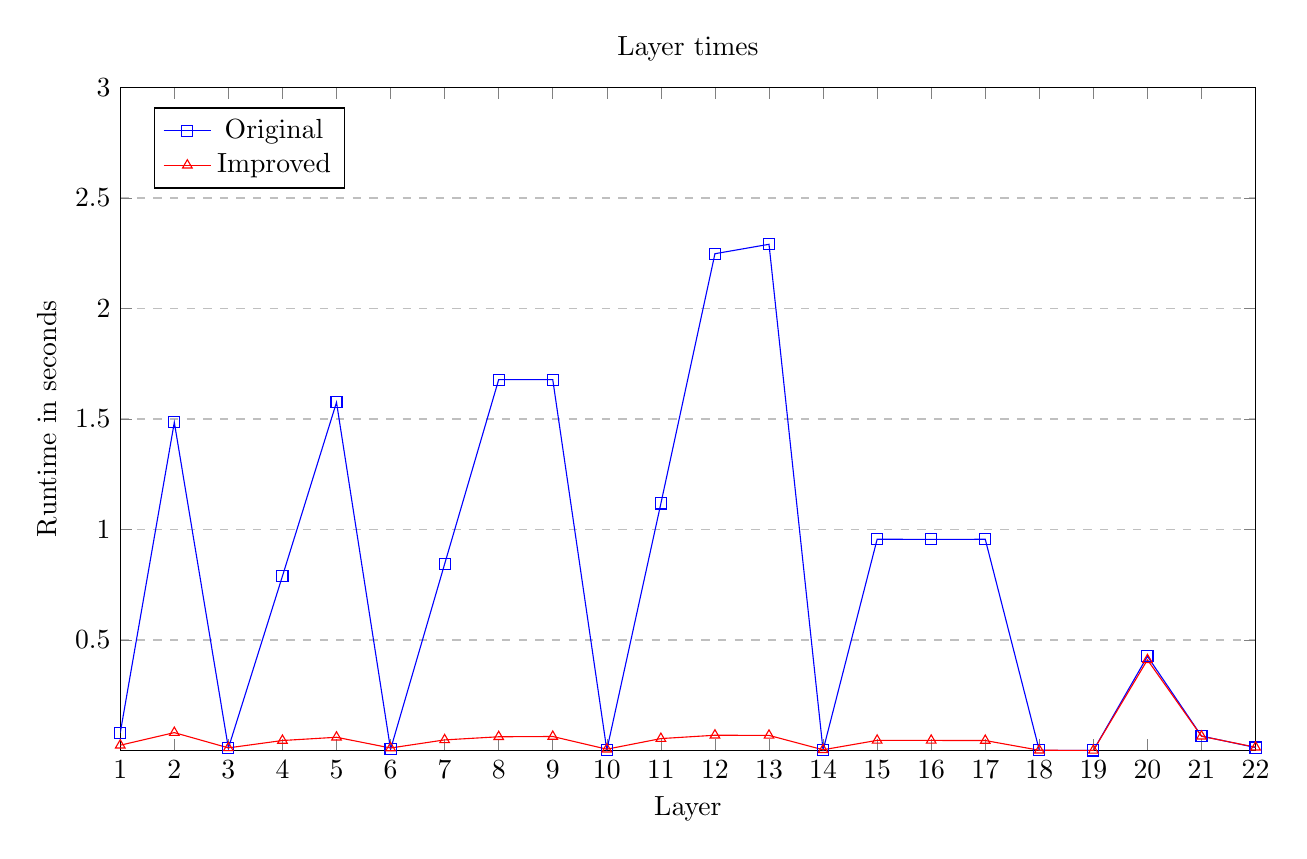
\begin{tikzpicture}
    \pgfplotsset{width=16cm,height=10cm}
    \begin{axis}[
        title={Layer times},
        xlabel={Layer},
        ylabel={Runtime in seconds},
        xmin=1, xmax=22,
        ymin=0, ymax=3,
        ytick={0.5,1,1.5,2,2.5,3},
        xtick={1,2,3,4,5,6,7,8,9,10,11,12,13,14,15,16,17,18,19,20,21,22},
        legend pos=north west,
        ymajorgrids=true,
        grid style=dashed,
    ]
    
    \addplot[
        color=blue,
        mark=square,
        ]
        coordinates {
          (1, 0.079800)(2, 1.484914)(3, 0.010580)(4, 0.788882)(5, 1.575170)
          (6, 0.004891)(7, 0.843748)(8, 1.678209)(9, 1.678326)(10, 0.002032)
          (11, 1.117702)(12, 2.248010)(13, 2.290603)(14, 0.000787)(15, 0.955651)
          (16, 0.955364)(17, 0.955552)(18, 0.000189)(19, 0.000040)(20, 0.426005)
          (21, 0.065086)(22, 0.013063)
        };
    
    \addplot[
        color=red,
        mark=triangle,
        ]
        coordinates {
          (1, 0.023599)(2, 0.080603)(3, 0.011564)(4, 0.044891)(5, 0.059594)
          (6, 0.011033)(7, 0.047659)(8, 0.061846)(9, 0.063014)(10, 0.005636)
          (11, 0.053596)(12, 0.068765)(13, 0.068054)(14, 0.002983)(15, 0.045573)
          (16, 0.045290)(17, 0.044787)(18, 0.000816)(19, 0.000112)(20, 0.41)
          (21, 0.064129)(22, 0.014556)
        };
        \legend{Original, Improved}
    \end{axis}
  \end{tikzpicture}
  \caption{Layer times of original and improved program}
  \label{layers}
\end{figure}

\bibliography{refs}
\end{document}